\chapter{ Regresión}
\label{sec:algoritmos}
Como se ha comentado previamente, se está trabajando sobre  un problema bastante peculiar, donde se intenta predecir distintas variables ordinales. Antes de comenzar con algoritmos más complejos, el primer enfoque para resolver el problema ha sido el de usar una media de cada variable a predecir. \\
Es cierto que usando este enfoque, estamos perdiendo información muy importante:  se está suponiendo que todas las variables son igualmente importantes, lo cual es una desventaja de esta aproximación al problema.
Por el contrario, este enfoque tiene la ventaja de estar usando algoritmos clásicos de regresión, proporcionando una salida más general, además de que usando este enfoque primero, descartamos la posibilidad de tener un conjunto de datos con mucho ruido o con un mal muestreo de los datos.\\
\linebreak
En esta sección vamos a explicar que algoritmos se han usado después del pre-procesamiento inicial.\\
Existe un teorema llamado\textbf{\textit{No-Free-Lunch}} que afirma no existe un algoritmo que resuelva los problemas de machine learning mejor que otro. Partiendo de esta idea, el objetivo principal de esta sección es el de comprobar el comportamiento de una serie de modelos e intentar mejorar el rendimiento de los mismos, añadiendo nuevos pasos a la etapa de pre-procesamiento y volviendo a entrenar los modelos que se han seleccionado. \\
\linebreak
\section{Rendimiento de modelos de regresión}
Para comprobar el comportamiento de los distintos modelos seleccionados, se han usado las siguientes \textbf{métricas de regresión}: \textit{\textbf{Coeficiente de determinación}} (se denota como $R^2$), \textit{\textbf{Desviación de Poisson}} y \textit{\textbf{Error cuadrático medio}}
\subsection{Coeficiente de determinación}
Se define como \textbf{coeficiente de determinación} como la proporción de la varianza total explicada por la variables independientes del modelo. Proporciona una indicación de como de bueno es un ajuste y por tanto, una medida de como de bueno es el modelo cuando predice nuevas muestras.\\
\linebreak
Matemáticamente, se define el coeficiente de determinación como:
\[
	R^2 (y, \hat{y}) = 1 - \frac{\sum_{i=1}^{n}(y_i - \hat{y}_i)^2}    {\sum_{i=1}^{n} (y_i - \overline{y})^2}
\]

Donde:
\begin{itemize}
	\item $y$ es el conjunto de valores reales para las variables objetivo.
	\item $\hat{y}$ es el valor predicho para los valores objetivo.
	\item $\hat{y}_i$ es la predicción de la  i-ésima muestra.
	\item $y_i$ es el valor real de la i-ésima muestra.
	\item $\overline{y} = \frac{1}{n} \sum_{i=1}^{n} y_i$.
	\item $n$ es el numero de muestras del conjunto.
\end{itemize}
insertar graficos explicando varianza,  etc
\subsection{Desviación de Poisson}
\subsection{Error cuadrático medio}
El error cuadrático medio de un estimador mide el promedio de los errores al cuadrado.  \\
Matemáticamente, se define el error cuadrático medio como:
\[
	MSE(y,\hat{y}) = \frac{1}{n} \sum_{i=1}^{n} (y_i - \hat{y}_i) ^2
\]
Donde:
\begin{itemize}
	\item $y$ es el conjunto de valores reales para las variables objetivo.
	\item $\hat{y}$ es el valor predicho para los valores objetivo.
	\item $\hat{y}_i$ es la predicción de la  i-ésima muestra.
	\item $y_i$ es el valor real de la i-ésima muestra.
	\item $n$ es el numero de muestras del conjunto.
\end{itemize}
\subsection{Conjuntos de validación}
\label{sec:validation}
Para ver el comportamiento de un modelo, no basta con definir un conjunto de entrenamiento para entrenar el modelo que se ha seleccionado y un conjunto de test para comprobar el comportamiento con datos que el algoritmo no conoce.  Aunque a primera vista esta parece una técnica correcta, tiene varios inconvenientes:
\begin{itemize}
	\item Cuando se ajustan los hiper-parámetros de los modelos,  se podría llegar a ajustar el modelo al conjunto de test, produciendo un sobre-ajuste.
	\item Solo se esta usando una parte de los datos para validar el modelo, nada asegura que el conjunto de test sea representativo del conjunto de datos con el que se está trabajando.
\end{itemize}
Para solventar estas y algunos otros problemas que que tiene esta metodología, se usa la \textbf{validación cruzada}.\\
\linebreak
En lugar de usar el conjunto de entrenamiento para entrenar un único modelo, se divide el conjunto de entrenamiento en $k$ partes, entrenando $k$ modelos usando $k-1$ subconjunto y usando el restante como de test. \\
\begin{figure}[H]
	\centering
	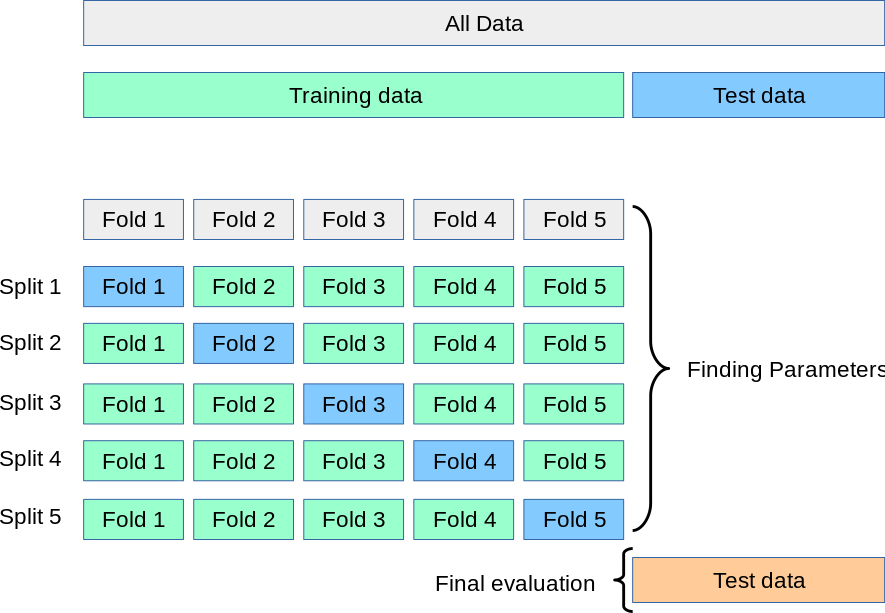
\includegraphics[scale=0.4]{grid_search_cross_validation.png}
	\caption{Ejemplo de validación cruzada con $k=5$}
	\label{fig:cross-validation}
\end{figure}
Como se aprecia en la figura \ref{fig:cross-validation},  se ha dividido el conjunto de datos en 5 conjuntos (folds), usando en cada iteración 4 para entrenar el modelo y uno para verificar con datos que el modelo no ha visto. Finalmente, se usa el conjunto de test (habiendo entrenado previamente el modelo con todo el conjunto de entrenamiento).
\subsection{Gráficos}
Además del uso de las métricas mencionadas previamente, se han creado las siguientes gráficas para visualizar los errores que esta haciendo un modelo en concreto. Esto ayuda a la toma de decisiones en fases siguientes.\\
Las gráficas que se han desarrollado son las siguientes:
\begin{itemize}
	\item Gráfico de dispersión de errores.
	\item Cantidad de errores por rango. (probablemente sea mejor cambiar este nombre, pero es el nombre que se me ocurrió)
\end{itemize}
El gráfico de dispersión de errores consiste en mostrar en la misma gráfica el valor real de las variables objetivo y el valor predicho por nuestro modelo. Esto nos permite ver como de juntos están las predicciones, identificando así en que zonas el algoritmo se está equivocando más frecuentemente.\\
\begin{figure}[H]
	\centering
	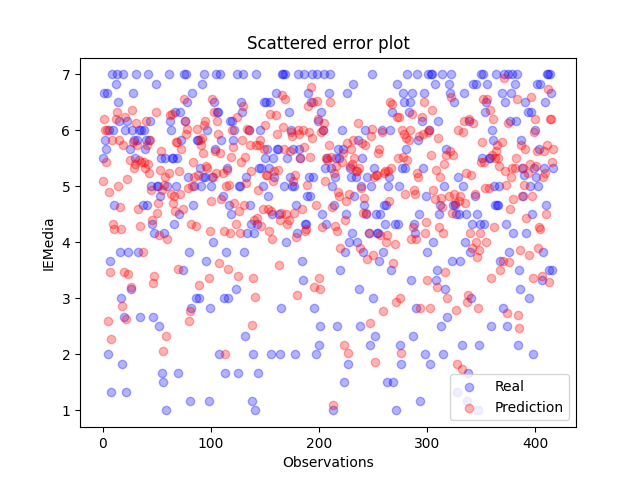
\includegraphics[scale=0.6]{scattered.png}
	\caption{Ejemplo de gráfico de dispersión de errores}
	\label{fig:scattered_example}
\end{figure}

El segundo gráfico consiste en lo siguiente:
Los modelos que han sido entrenados están prediciendo valores medios. El proceso seguido para realizar estos gráficos ha sido el de obtener los valores redondeados tanto de la predicción como del valor real. Si el valor redondeado de la predicción y del dato real son distintos, se ha considerado como error.  Sumando estos errores, se puede generar un gráfico de barras como el siguiente para tener una visión más clara de en que zonas de la predicción el algoritmo esta funcionando peor:
\linebreak
\begin{figure}[H]
	\centering
	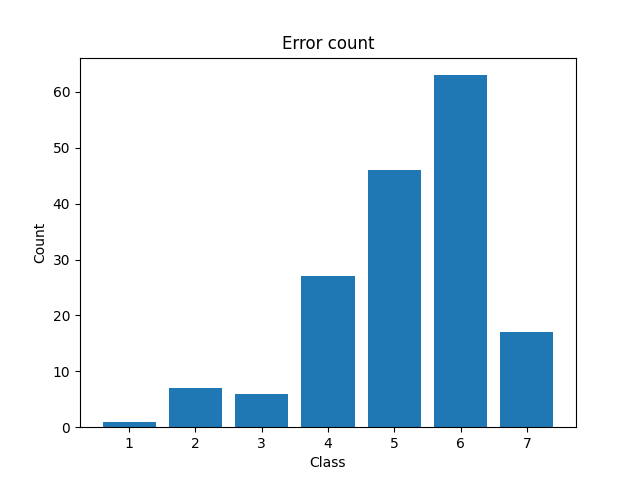
\includegraphics[scale=0.6]{error_hist.png}
	\caption{Ejemplo de gráfico de errores por rango}
	\label{fig:error_hist_example}
\end{figure}
\section{Modelos de regresión}
\subsection{Árboles de decisión}
\label{alg:dec_tree}
Los árboles de decisión son modelos que predicen la variable objetivo usando reglas del tipo \textit{si variable cumple condición entonces } inferidas a partir de los datos con los que se entrena el algoritmo.\\
Los árboles de decisión ofrecen ciertas ventajas:
\begin{enumerate}
	\item Son modelos fáciles de interpretar y pueden ser visualizados.
	\item Son capaces de trabajar con variables categóricas y numéricas.
	\item introducir alguna ventaja más
\end{enumerate}
Sin embargo, también presentan ciertas desventajas:
\begin{enumerate}
	\item Modelos que tienden al sobre-aprendizaje.
	\item No soportan valores perdidos.
	\item No trabajan bien con conjuntos de datos des-balanceados.
\end{enumerate}
Se ha seleccionado este modelo debido a que puede proporcionar información extra sobre conjunto de datos como la importancia de variables, que puede ser interesante a la hora de hacer uso de la información obtenida por los modelos.
\subsubsection*{Procesado de datos}
Antes de ejecutar la fase de entrenamiento, hay que modificar los datos para adaptarlos a las limitaciones del modelo. En este caso,  los Árboles de Decisión no admiten valores perdidos y debido a ciertas limitaciones de la librería que se está usando,  no son capaces de trabajar con variables categóricas, aunque generalmente si son capaces de trabajar con este tipo de variables..\\
Las modificaciones que se han hecho previamente son: (por orden)
\begin{enumerate}
	\item \textbf{Imputación de valores perdidos}
	\item \textbf{Transformación de variables categóricas a numéricas}
\end{enumerate}
Por este motivo, se ha tenido que introducir una fase extra transformando las variables categóricas en numéricas.
\subsubsection*{Resultados}
\label{sec:res_tree}
Antes de mostrar los resultados, hay que destacar que cuando se entrena un árbol de decisión sin limitar los parámetros, este va a seguir separando los datos de entrenamiento hasta que no pueda realizar más divisiones. Para encontrar el árbol óptimo, primero se ha entrenado el árbol por defecto y se han obtenido los parámetros. Esos parámetros se han establecido como limite, se han entrenado varios árboles con distintos parámetros (sin superar el límite establecido por el primer modelo) y se ha escogido el que mejores resultados obtenía. Los parámetros que mejor resultados dieron son: \\
\begin{itemize}
	\item \textbf{Profundidad máxima:} Limita la profundidad (cantidad de preguntas) del árbol. El mejor valor ha sido \textbf{8}
	\item \textbf{Máximo número de hojas:} Máximo numero de hojas (grupos en el último nivel de una rama). El mejor valor ha sido \textbf{16}
\end{itemize}
En esta sección se va a exponer los resultados obtenidos usando  \textbf{Árboles de Decisión}.\\
La siguiente tabla expone los resultados obtenidos en validación:
\begin{table}[htbp]
	\centering
	\begin{tabular}{|c|c|c|c|c}
		\cline{1-4}
		FOLD   & R2    & Poisson Deviance & MSE   \\ \cline{1-4}
		Fold 0 & 0.678 & 0.211            & 0.886 \\ \cline{1-4}
		Fold 1 & 0.661 & 0.206            & 0.884 \\ \cline{1-4}
		Fold 2 & 0.629 & 0.239            & 0.98  \\ \cline{1-4}
		Fold 3 & 0.67  & 0.191            & 0.8   \\ \cline{1-4}
		Fold 4 & 0.636 & 0.211            & 0.933 \\ \cline{1-4}
		Fold 5 & 0.655 & 0.212            & 0.897 \\ \cline{1-4}
		Train  & 0.748 & 0.156            & 0.659 \\ \cline{1-4}
		Test   & 0.69  & 0.196            & 0.815 \\ \cline{1-4}
	\end{tabular}
	\caption{Árbol de decisión: Profundidad 8, número máximo de hojas 16}
	\label{tab:tree_res}
\end{table}
La siguiente figura muestra el gráfico de dispersión de errores:\\
\begin{figure}[H]
	\centering
	\includegraphics[scale=0.8]{src/scattered_error_dtree.png}
	\caption{Gráfico de dispersión de errores}
	\label{fig:tree_scattered}
\end{figure}
Continuando con las gráficas, e continuación se muestra una gráfica con el conteo de errores por clase:
\begin{figure}[H]
	\centering
	\includegraphics[scale=0.8]{src/error_hist_dtree.png}
	\caption{Conteo de errores}
	\label{fig:tree_error_plot}
\end{figure}
\subsubsection*{Representación}
Como se mencionó en la sección \textbf{\ref{alg:dec_tree}-\nameref{alg:dec_tree}}, los árboles de decisión tienen la ventaja de que pueden representarse fácilmente. \\
En este caso, vamos a usar una representación gráfica del árbol, las reglas que ha obtenido el árbol y las variables más importantes.\\
\linebreak
La siguiente figura muestra la representación gráfica del árbol de decisión entrenado:\\
\linebreak
\begin{figure}[H]
	\centering
	\includegraphics[scale=0.2]{src/dtree_plot.png}
	\caption{Árbol de decisión}
	\label{fig:decission_tree1}
\end{figure}
\pagebreak
Por ultimo, estas son las 10 variables que el modelo consideró con más relevancia. El valor asociado a cada variable es la \textbf{importancia Gini}:
\begin{figure}[H]
	\centering
	\includegraphics[scale=0.25]{src/feature_importance_dtree}
	\caption{10 variables más importantes segun AD}
	\label{fig:feature_dtree}
\end{figure}
Volviendo a la documentación proporcionada para comprobar el significado de esos valores:
\begin{itemize}
	\item \textbf{AE5:} Pregunta  5 sobre Actitudes financieras empresariales. Valor $0.735667$
	\item \textbf{AcMedia:} Variable global de Actitud emprendedora. Valor $0.156046$
	\item \textbf{SE2:} Estoy preparado para iniciar una empresa viable. Valor $0.037300$
	\item \textbf{SE5:} Conozco cómo desarrollar un proyecto empresarial. Valor $0.014692$
	\item \textbf{NS1:} Mi familia aprobaría el que yo decidiese crear una empresa. Valor $0.012393$
	\item \textbf{Beca:} Tiene beca el encuestado. Valor $0.008256$
	\item \textbf{Nota:} Nota media del expediente académico hasta la fecha de la encuesta sobre 10 puntos. Valor $0.008034$
	\item \textbf{BA3.f:} En los últimos 12 meses, ¿has ahorrado personalmente algún dinero de alguna de las siguientes formas, independientemente de si aún dispones del dinero? Han contestado las opciones a, c, d, e, f, g (en casa, en cuenta de ahorro, darlo a la familia, productos de inversión, de otro modo). Valor $0.007389$
	\item \textbf{CEF19:} Pregunta sobre Conocimientos financieros empresariales. Valor $0.007202$
	\item \textbf{AE7:} Pregunta 7 sobre Actitudes financieras empresariales. Valor $0.006518$
\end{itemize}
De las columnas \textit{AEx} y \textit{CEFx} no hay información en la documentación, unicamente se menciona que son una serie de preguntas relacionadas con actitudes financieras empresariales y sobre conocimientos financieros empresariales respectivamente.
\subsection{Random Forest}
\label{sec:rf}
Random Forest es un modelo  combinado de aprendizaje que puede usarse para clasificación y/o regresión. Random Forest consiste en un conjunto de árboles de decisión que operan juntos. Una vez que cada árbol dentro del Random Forest realiza una predicción, se escoge la predicción con más votos. \\ Se ha escogido este modelo ya que como se comprobó en la sección \textbf{\ref{alg:dec_tree}-\nameref{alg:dec_tree}}, los árboles de decisión dieron buenos resultados
\linebreak
Para que Random Forest funciona bien, hay que asegurar que los distintos árboles que lo forman tengan una baja \textbf{correlación} entre ellos. Esto quiere decir que los árboles tienen que diferir y proporcionar predicciones distintas, de esta manera, si hay un conjunto de  árboles que da una predicción malas, puede haber otro conjunto que vaya en la dirección correcta. \\
\linebreak
Los Árboles de Decisión son modelos que son muy sensibles a los datos con los que se ha entrenado, por lo que cualquier cambio en los datos de entrenamiento puede hacer que cambie una predicción. Random Forest hace uso de esta peculiaridad de los árboles de decisión.
En el momento de entrenar los distintos árboles, en vez de usar subconjuntos del conjunto de entrenamiento se usan $N$ conjuntos del mismo tamaño que el conjunto de entrenamiento obtenidos usando un \textbf{muestreo con reemplazo}. Una vez que se tienen los distintos conjuntos, se entrena cada conjunto con un árbol. Este proceso se conoce como \textbf{bagging}.\\
\linebreak
Una peculiaridad más que tiene Random Forest es la forma con la que los árboles seleccionan la variable que van a usar para dividir el conjunto de datos. Estos no eligen la variable en función de un criterio concreto, si no que eligen la variable usando un conjunto aleatorio de las características.  Esto fuerza a que los árboles sean mas diferentes entre ellos, bajando la correlación entre los árboles que forman el modelo.
\subsubsection*{Procesado de datos}
Al igual que los árboles de decisión, se ha hecho una imputación de valores perdidos y se ha transformado las variables categóricas a numéricas debido a limitación que hay en la librería usada.
\pagebreak
\subsubsection*{Resultados}
Antes de mostrar los resultados, estos son los parámetros que se han usado al entrenar el modelo:
\begin{itemize}
	\item \textbf{max\_features}:  Número de variables que se van a escoger de manera aleatoria: $\frac{1}{3}$ del número de variables.
	      \item\textbf{n\_estimators}: Número de árboles que forman el Random Forest: $500$
\end{itemize}
En la siguiente tabla, se muestra el resultado para obtenidos en validación y en test:
\linebreak
\begin{table}[H]
	\centering
	\begin{tabular}{|c|c|c|c|c}
		\cline{1-4}
		FOLD   & R2    & Poisson Deviance & MSE   \\ \cline{1-4}
		Fold 0 & 0.767 & 0.155            & 0.642 \\ \cline{1-4}
		Fold 1 & 0.775 & 0.137            & 0.586 \\ \cline{1-4}
		Fold 2 & 0.741 & 0.17             & 0.684 \\ \cline{1-4}
		Fold 3 & 0.736 & 0.151            & 0.64  \\ \cline{1-4}
		Fold 4 & 0.747 & 0.15             & 0.649 \\ \cline{1-4}
		Fold 5 & 0.753 & 0.153            & 0.64  \\ \cline{1-4}
		Train  & 0.967 & 0.023            & 0.087 \\ \cline{1-4}
		Test   & 0.769 & 0.149            & 0.606 \\ \cline{1-4}
	\end{tabular}
	\caption{Random Forest}
	\label{tab:res_random_forest}
\end{table}
La siguiente figura muestra el gráfico de dispersión de errores:\\
\linebreak
\begin{figure}[H]
	\centering
	\includegraphics[scale=0.7]{src/scattered_error_rf.png}
	\caption{Gráfico de dispersión de errores}
	\label{fig:rf_scattered}
\end{figure}
Continuando con las gráficas, e continuación se muestra una gráfica con el conteo de errores por clase:
\begin{figure}[H]
	\centering
	\includegraphics[scale=0.7]{src/error_hist_rf.png}
	\caption{Conteo de errores}
	\label{fig:rf_error_plot}
\end{figure}
Para finalizar, esta es la lista de las 10 variables más importantes que ha obtenido Random Forest:
\begin{figure}[H]
	\centering
	\includegraphics[scale=0.6]{src/feature_importance_rf}
	\caption{10 variables más importantes según RF}
	\label{fig:feature_rf}
\end{figure}
Volviendo a la documentación, esta es la explicación para cada variable:
\begin{itemize}
	\item\textbf{AE5:} Pregunta  5 sobre Actitudes financieras empresariales. Valor = $0.246364$
	\item\textbf{AcMedia:} Variable global de Actitud emprendedora. Valor = $0.220202$
	\item\textbf{AC2:} Ser emprendedor es una salida profesional atractiva para mí. Valor = $0.072907$
	\item\textbf{AC4:}Ser emprendedor supondría una gran satisfacción para mí. Valor = $0.065776$
	\item\textbf{AC3:} Si tuviera la oportunidad y los recursos, me gustaría iniciar una empresa. Valor = $0.041642$
	\item\textbf{SEMedia:} Variable global de Autoeficacia emprendedora. Valor = $0.022872$
	\item\textbf{SE2:} Estoy preparado para iniciar una empresa viable. Valor = $0.019630$
	\item\textbf{AC1:} Ser emprendedor implica más ventajas que desventajas para mí. Valor = $0.019396$
	\item\textbf{NS1:} Mi familia aprobaría el que yo decidiese crear una empresa. Valor = $0.014467$
	\item\textbf{Nota:} Nota media del expediente académico hasta la fecha de la encuesta sobre 10 puntos. Valor = $0.012254$
\end{itemize}
\subsection{KNN}
\label{alg:knn}
KNN (\textit{K Nearest Neighbors}) es un algoritmo supervisado basado en instancias. Este algoritmo no aprende un modelo si no que almacena todas las muestras de entrenamiento y cuando hay que predecir una nueva ejemplo, el algoritmo usa las muestras almacenadas calculando la distancia a cada muestra y obteniendo los K vecinos más cercanos y usando las valores reales de los vecinos seleccionados, asigna una predicción al ejemplo a predecir, generalmente asignando aquella clase con más "votos".\\
\linebreak
Para medir la distancia entre dos muestras, KNN puede usar una gran cantidad métricas, las más comunes son:
\begin{itemize}
	\item \textbf{Distancia euclidiana:} Definida como $\sqrt{\sum(x_1 - x_2)^2}$
	\item \textbf{Distancia Manhattan:} Definida como $\sum|x_1 - x_2|$
	\item \textbf{Distancia Minkowski:} Definida como $(\sum|x_1 - x_2|^p)^{\frac{1}{p}}$, siendo P un entero positivo
\end{itemize}
La implementación del algoritmo KNN de ScikitLearn usa por defecto la distancia \textbf{Minkowski}. Esta tiene la peculiaridad de que cambiando el parámetro $p$ puede usarse la distancia euclidiana ($p=2$) o la distancia Manhattan ($p=1$)
\subsubsection*{Procesado de datos}
KNN es un algoritmo que depende de la distancia entre dos muestras, esto implica que si una caracteristica del conjunto de datos que se esta usando tiene un rango \textbf{mayor} que otra, esa característica aportará más al cálculo de la distancia, cuando no necesariamente debe de ser así. Por ese motivo, este algoritmo necesita que el conjunto de datos esté \textbf{normalizado} en el momento de entrenar.\\
\linebreak
Este algoritmo, a parte de necesitar que los datos estén normalizados, no admite valores perdidos y variables categóricas.

\subsubsection*{Resultados}
Antes de mostrar los resultados, estos son los parámetros que se han usado al entrenar el algoritmo:
\begin{itemize}
	\item \textbf{K:} Número de vecinos: 5
	\item \textbf{Métrica:} Distancia usada: Minkowski con $P=2$ (distancia euclidiana).
\end{itemize}
En la siguiente tabla, se muestra el resultado para obtenidos en validación y en test:
\linebreak
\begin{table}[H]
	\centering
	\begin{tabular}{|c|c|c|c|c}
		\cline{1-4}
		FOLD   & R2    & Poisson Deviance & MSE   \\ \cline{1-4}
		Fold 0 & 0.47  & 0.356            & 1.46  \\  \cline{1-4}
		Fold 1 & 0.407 & 0.378            & 1.545 \\  \cline{1-4}
		Fold 2 & 0.449 & 0.362            & 1.457 \\  \cline{1-4}
		Fold 3 & 0.435 & 0.329            & 1.372 \\  \cline{1-4}
		Fold 4 & 0.467 & 0.321            & 1.367 \\  \cline{1-4}
		Fold 5 & 0.446 & 0.349            & 1.44  \\  \cline{1-4}
		Train  & 0.653 & 0.227            & 0.907 \\ \cline{1-4}
		Test   & 0.527 & 0.301            & 1.242 \\ \cline{1-4}
	\end{tabular}
	\caption{KNN: $K=5$, métrica Minkowski con $P=2$}
	\label{tab:knn_res}
\end{table}
La siguiente figura muestra el gráfico de dispersión de errores:
\begin{figure}[H]
	\centering
	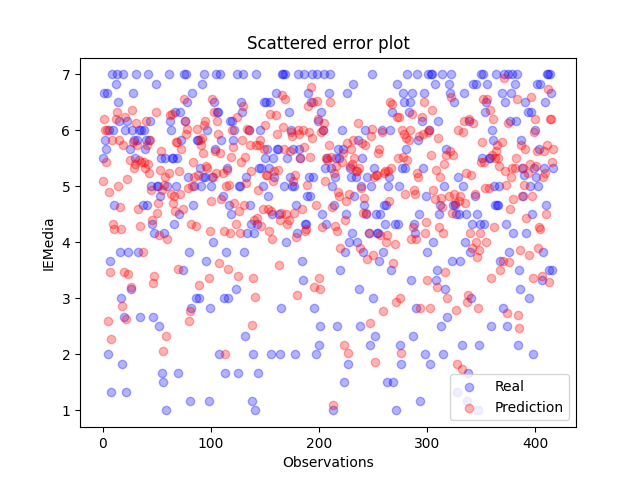
\includegraphics[scale=0.8]{src/scattered_error_knn.png}
	\caption{Gráfico de dispersión de errores}
	\label{fig:knn_scattered}
\end{figure}
Continuando con las gráficas, e continuación se muestra una gráfica con el conteo de errores por clase:\\
\linebreak
\begin{figure}[H]
	\centering
	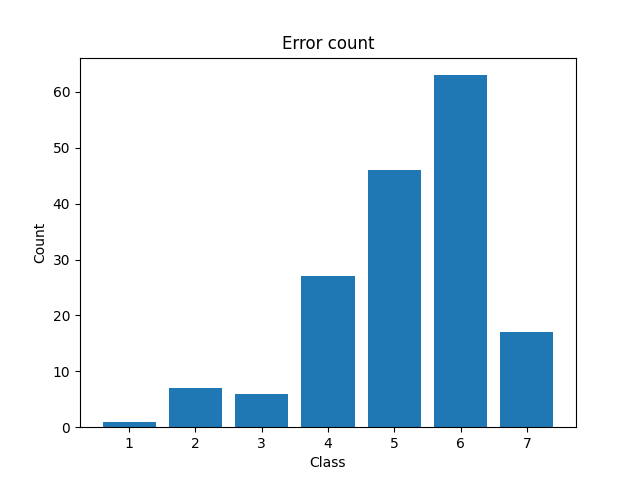
\includegraphics[scale=0.8]{src/error_hist_knn.png}
	\caption{Conteo de errores}
	\label{fig:knn_error_plot}
\end{figure}
\subsection{SVM}
\label{sec:svm}
Maquina de soporte de vectores (Support Vector Machines) es un modelo de aprendizaje supervisado cuyo objetivo es encontrar un hiper-plano dentro de un espacio de  $N$ dimensiones ($N$ es el número de características del conjunto de datos) que clasifique las muestras de dentro del espacio en distintas clases.  Originalmente, se diseñó para clasificación binaria, pero en la actualidad este algoritmo se ha adaptado para regresión, clasificación multi-clase y  multi-etiqueta\\
\linebreak
Pueden existir muchos hiper-planos que separen los puntos del espacios en distintas clases. El objetivo de SVM es encontrar aquel hiper-plano con mayor \textbf{margen} (distancia entre puntos de distintas clases),  ya que incrementa la posibilidad de clasificar correctamente muestras que no se han usado en entrenamiento al disponer de un margen mayor de error. Los vectores soporte son aquellas observaciones del conjunto de datos que definen el hiper-plano. Idealmente, estas o\\
\begin{figure}[H]
	\centering
	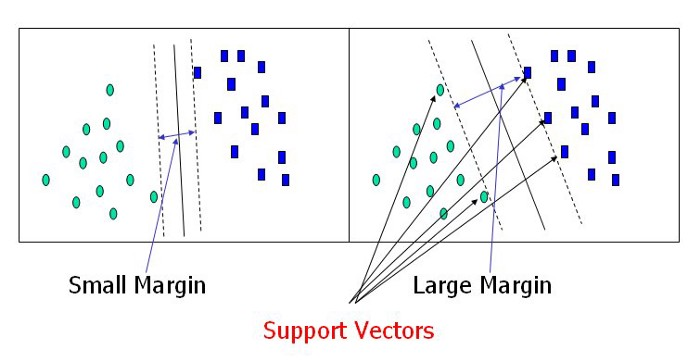
\includegraphics[scale=0.5]{svm}
	\caption{Ejemplo de SVM en dos dimensiones}
	\label{fig:svm}
\end{figure}
\subsubsection*{Procesado de datos}
SVM son modelos con una fuerte base matemática, por lo que son modelos que no pueden ser entrenados usando variables categóricas.
Las modificaciones que se han hecho previamente son: (por orden)
\begin{enumerate}
	\item \textbf{Imputación de valores perdidos.}
	\item \textbf{Escalado de valores numéricos.}
	\item \textbf{Transformación de variables categóricas a numéricas.}
\end{enumerate}
\subsubsection*{Resultados}
A continuación se muestra una tabla con los resultados obtenidos por SVM en el conjunto de validación y en el conjunto de test:
\begin{table}[H]
	\centering
	\begin{tabular}{|c|c|c|c|c}
		\cline{1-4}
		FOLD   & R2    & Poisson Deviance & MSE   \\ \cline{1-4}
		Fold 0 & 0.671 & 0.236            & 0.906 \\ \cline{1-4}
		Fold 1 & 0.718 & 0.186            & 0.734 \\ \cline{1-4}
		Fold 2 & 0.728 & 0.185            & 0.72  \\ \cline{1-4}
		Fold 3 & 0.691 & 0.192            & 0.75  \\ \cline{1-4}
		Fold 4 & 0.697 & 0.193            & 0.776 \\ \cline{1-4}
		Fold 5 & 0.701 & 0.198            & 0.777 \\ \cline{1-4}
		Train  & 0.894 & 0.076            & 0.276 \\ \cline{1-4}
		Test   & 0.737 & 0.173            & 0.691 \\ \cline{1-4}
	\end{tabular}
	\caption{SVM: Tolerancia $1^{-3}$, Kernel RBF, $C=1$}
	\label{tab:svm_res}
\end{table}
La siguiente figura muestra el gráfico de dispersión de errores:
\begin{figure}[H]
	\centering
	\includegraphics[scale=0.8]{src/scattered_error_svr.png}
	\caption{Gráfico de dispersión de errores}
	\label{fig:svr_scattered}
\end{figure}
Continuando con las gráficas, e continuación se muestra una gráfica con el conteo de errores por clase:\\
\linebreak
\begin{figure}[H]
	\centering
	\includegraphics[scale=0.8]{src/error_hist_svr.png}
	\caption{Conteo de errores}
	\label{fig:svr_error_plot}
\end{figure}
\subsection{XGBoost}
Extreme Gradient Boosting  es un método de aprendizaje combinado basado en árboles de decisión.\\
A diferencia de Random Forest (que también es un método combinado basado en árboles de decisión), XGBoost hace uso de técnicas de \textit{Gradient Boosting}  frente a Random Forest que hace uso de \textit{Bagging} para entrenar los modelos que lo forman. (\ref{sec:rf}-\nameref{sec:rf}).\\
\linebreak
\textit{Boosting} se basa en la unión de varios modelos débiles para formar un modelo que en conjunto. Estos modelos débiles se van entrenando de forma iterativa, adaptando los parámetros del modelo en cada iteración,  teniendo en cuenta que estos modelos no deben aumentar en complejidad y deben mantener un rendimiento mínimo (idealmente, mejor que un clasificador aleatorio).\\
\linebreak
\textit{Grandient Boosting} es un caso especial de \textit{Boosting} en el que se hace uso del algoritmo  \textbf{Gradiente Descendente} para minimizar los errores de los modelos simples.\\
\linebreak
Finalmente, XGBoost funciona añadiendo secuencialmente Árboles de Decisión, de tal manera que cada árbol reduzca el error de los previos aprendiendo de los errores que han cometido los árboles anteriores.
\subsubsection*{Procesado de datos}
El pre-procesado aplicado para este modelo ha sido similar al usado en Árboles de Decisión:
\begin{enumerate}
	\item \textbf{Imputación de valores perdidos}
	\item \textbf{Transformación de variables categóricas a numéricas}
\end{enumerate}
\subsubsection*{Resultados}
A continuación se muestra una tabla con los resultados obtenidos por \textbf{XGBoost} en los conjuntos de validación, train y test:
\begin{table}[H]
	\centering
	\begin{tabular}{|c|c|c|c|c|}
		\cline{1-4}
		FOLD   & R2    & Poisson Deviance & MSE   \\ \cline{1-4}
		Fold 0 & 0.726 & 0.186            & 0.754 \\ \cline{1-4}
		Fold 1 & 0.734 & 0.165            & 0.693 \\ \cline{1-4}
		Fold 2 & 0.71  & 0.196            & 0.766 \\ \cline{1-4}
		Fold 3 & 0.723 & 0.16             & 0.671 \\ \cline{1-4}
		Fold 4 & 0.744 & 0.157            & 0.658 \\ \cline{1-4}
		Fold 5 & 0.727 & 0.173            & 0.708 \\ \cline{1-4}
		Train  & 0.991 & 0.005            & 0.024 \\ \cline{1-4}
		Test   & 0.741 & 0.162            & 0.68  \\ \cline{1-4}
	\end{tabular}
	\caption{Métricas de XGBoost con}
	\label{tab:xgboost}
\end{table}
La siguiente figura muestra el gráfico de dispersión de errores:
\begin{figure}[H]
	\centering
	\includegraphics[scale=0.8]{src/scattered_error_xgboost.png}
	\caption{Gráfico de dispersión de errores para XGBoost}
	\label{fig:xgboost_scattered}
\end{figure}
Finalizando con las gráficas, a continuación se muestra una gráfica con el conteo de errores por clase:
\begin{figure}[H]
	\centering
	\includegraphics[scale=0.8]{src/error_hist_xgboost.png}
	\caption{Conteo de errores}
	\label{fig:xgboost_error_plot}
\end{figure}

\subsection{Perceptrón multicapa}
El Perceptrón Multicapa es un modelo de aprendizaje supervisado basada en red neuronales artificiales y haciendo uso del algoritmo \textbf{Perceptrón}.\\
\linebreak
El Perceptrón es un algoritmo de aprendizaje supervisado para clasificación binaria. Es un clasificador linear que funciona iterando sobre cada muestra del conjunto de datos hasta calcular un hiper-plano que separe el conjunto de datos. Los pasos de este algoritmo son:
\begin{enumerate}
	\item Establecer un plano inicial (generalmente de manera aleatoria ).
	\item Por cada muestra del conjunto de datos, si la muestra está mal clasificada, se modifican los pesos que definen el hiper-plano para clasificar correctamente esa muestra.
	\item El paso anterior se repite hasta que todas las muestras estén bien clasificadas ó no se haya hecho ninguna modificación. Por lo general, también se añade un número máximo de iteraciones que se van a realizar.
\end{enumerate}
Este algoritmo tiene una limitación muy fuerte: No puede resolver problemas no lineales (incluso funciones sencillas como la \textit{XOR}). \\
\linebreak
Para afrontar este problema, se propuso el usar una combinación de perceptrones siguiendo una estructura de red neuronal, consiguiendo así un modelo capaz de resolver problemas no lineales. Estas redes neuronales tienen al menos 3 capas:
\begin{itemize}
	\item Capa de entrada: Está formada por las primeras neuronas que forman la red y se encargan de introducir los datos a la red.
	\item Capa/s oculta: Son las capas de la zona media de la red y son las encargadas del procesamiento de los datos para formar el modelo.
	\item Capa de salida: Dan el valor de salida del modelo.
\end{itemize}
\begin{figure}[H]
	\centering
	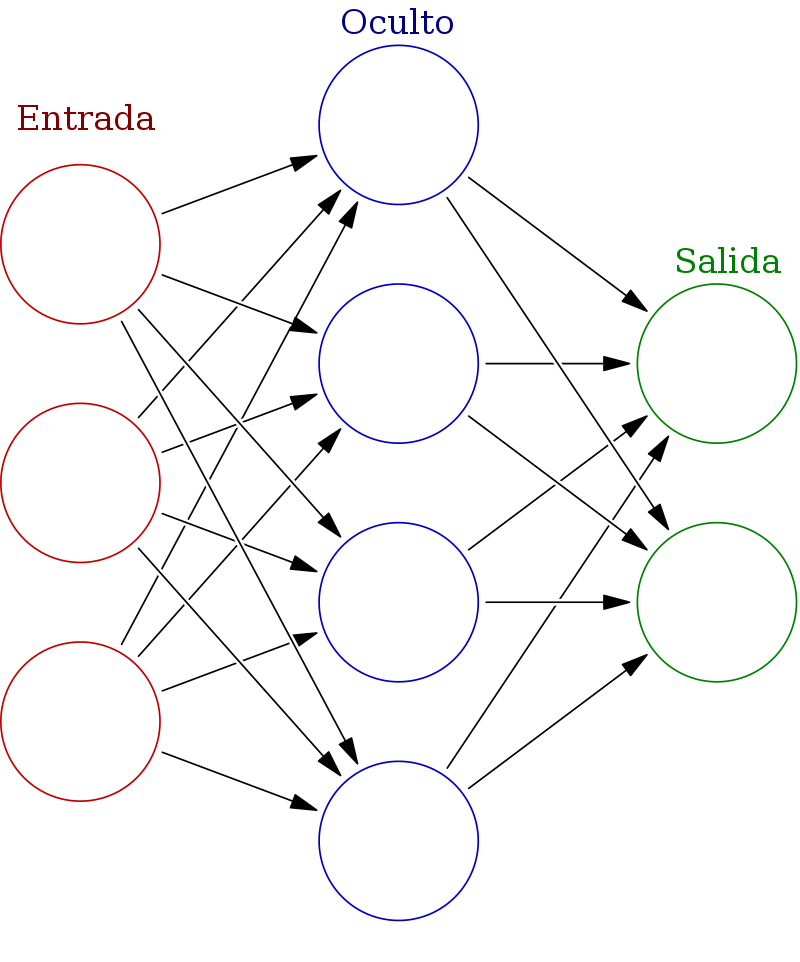
\includegraphics[scale=0.3]{rnn}
	\caption{Ejemplo de Red Neuronal con 1 capa oculta}
	\label{fig:rnn}
\end{figure}
Un elemento fundamental de las Redes Neuronales es el algoritmo de \textit{back-propagation}. Este algoritmo usa el error obtenido en las capas de salida y este era propagado hacia cada neurona anterior (de ahí el nombre de \textit{back-propagation}), ajustando así el peso calculado por cada neurona en función del comportamiento del modelo en la iteración anterior.
\subsubsection*{Procesado de datos}
Como se puede apreciar, el MLP son algoritmos con una fuerte base matemática, por lo que no son capaces de ser entrenados usando variables categóricas. Las modificaciones que se han hecho sobre el conjunto de datos son las siguientes:
\begin{enumerate}
	\item \textbf{Imputación de valores perdidos.}
	\item \textbf{Escalado de valores numéricos.}
	\item \textbf{Transformación de variables categóricas a numéricas.}
\end{enumerate}
\subsubsection*{Resultados}
En esta sección se va a mostrar los resultados obtenidos por el Perceptrón Multi-capa. \\
\linebreak
En esta tabla, se puede observar el rendimiento del modelo en los conjuntos de validación, entrenamiento y test:
\begin{table}[H]
	\centering
	\begin{tabular}{|c|c|c|c|c}
		\cline{1-4}
		FOLD   & R2    & Poisson Deviance & MSE   \\\cline{1-4}
		Fold 0 & 0.557 & 0.321            & 1.221 \\\cline{1-4}
		Fold 1 & 0.566 & 0.274            & 1.13  \\\cline{1-4}
		Fold 2 & 0.586 & 0.269            & 1.096 \\\cline{1-4}
		Fold 3 & 0.412 & 0.291            & 1.427 \\\cline{1-4}
		Fold 4 & 0.488 & 0.303            & 1.313 \\\cline{1-4}
		Fold 5 & 0.522 & 0.292            & 1.237 \\\cline{1-4}
		Train  & 0.999 & 0.0              & 0.002 \\\cline{1-4}
		Test   & 0.616 & 0.27             & 1.007 \\\cline{1-4}
	\end{tabular}
	\caption{Perceptrón Multicapa: 1 capa oculta con 100 neuronas, 500 iteraciones max}
	\label{tab:mlp_res}
\end{table}
La siguiente figura muestra el gráfico de dispersión de errores:
\begin{figure}[H]
	\centering
	\includegraphics[scale=0.8]{src/scattered_error_MLP.png}
	\caption{Gráfico de dispersión de errores}
	\label{fig:mlp_scattered}
\end{figure}
Continuando con las gráficas, e continuación se muestra una gráfica con el conteo de errores por clase:\\
\linebreak
\begin{figure}[H]
	\centering	\includegraphics[scale=0.8]{src/error_hist_MLP.png}
	\caption{Conteo de errores}
	\label{fig:mlp_error_plot}
\end{figure}
\section{Conclusiones}
Se ha observado que los modelos basados en Árboles de Decisión y Random Forest han tenido un buen comportamiento, por lo que se ha optado por seguir haciendo uso de ellos en secciones siguientes. XGBoost, tiene unos resultados ligeramente peores respecto a Random Forest pero con un comportamiento similar, fallando considerable en valores altos de intención emprendedora media). Como XGBoost no esta aportando nada nuevo, por ahora se va a descartar.\\
\linebreak
SVR se ha comportado casi al nivel de modelos como XGBoost o Random Forest. Por ahora, no se va a descartar su uso, ya que introduciendo el conocimiento que se ha obtenido usando modelos como Random Forest o árboles de decisión se podría mejorar el rendimiento.\\
\linebreak
Los resultados obtenidos por  KNN demuestran que este algoritmo no funciona bien con el conjunto de datos que se está usando. La razón más probable por la que KNN obtuvo estos resultados, es que hay relaciones entre las variables que KNN no es capaz de detectar, al comparar únicamente la distancia característica por característica. Debido al bajo desempeño que se ha obtenido al usar KNN, va a ser descartado de las siguientes fases.\\
\linebreak
Respecto al Perceptrón Multicapa, ya que el rendimiento en comparación con otros modelos probados y debido al enorme coste de entrenamiento que pueden llegar a tener, se ha decidido no continuar haciendo uso de este modelo.\\
\linebreak
Como ya se ha mencionado, los modelos basados en árboles de decisión son capaces de obtener la importancia de las características. A continuación se muestran las gráficas de nuevo para facilitar la comparación:
\begin{figure}[H]
	\centering
	\includegraphics[scale=0.5]{src/feature_importance_dtree}
	\caption{10 variables más importantes según árboles de decisión}
	\label{fig:feature_dtree2}
\end{figure}
\begin{figure}[H]
	\centering
	\includegraphics[scale=0.5]{src/feature_importance_rf}
	\caption{10 variables más importantes según RF}
	\label{fig:feature_rf2}
\end{figure}
Como se ve en las figuras, vemos que hay dos variables que \textbf{ambos} algoritmos han dado como más importantes:
\begin{itemize}
	\item\textbf{AE5:} Pregunta  5 sobre Actitudes financieras empresariales.
	\item\textbf{AcMedia:} Variable global de Actitud emprendedora.
\end{itemize}
Repasando los resultados, se puede apreciar que a todos los algoritmos usados les está costando predecir correctamente los valores altos para la intención emprendedora media (véase figura \ref{fig:rf_error_plot}). Este comportamiento ha sido constante para cada algoritmo usado. La causa de este comportamiento puede ser que a medida que se incrementa el valor de intención emprendedora media, los datos son menos dispersos y a los algoritmos les está costando distinguir entre varios valores cercanos. Este comportamiento se puede apreciar en los gráficos de dispersión de errores que se han mostrado previamente.
\pagebreak
\section{Muestreo de datos}
Una vez se ha comprobado el rendimiento de los distintos modelos que se han seleccionado, se va a intentar mejorarlo añadiendo nuevas etapas extra al procesamiento de datos antes de entrenar los modelos.
\newline
Como se ha podido observar en la primera iteración, todos los algoritmos se están equivocando en valores altos. Para intentar reducir el ruido, se va tratar el conjunto de datos haciendo \textbf{under-sampling}.\\
Under-Sampling (se podría traducir como \textit{muestreo}) es una técnica para reducir el ruido del conjunto de datos eliminando algunas muestras del conjunto de datos.\\
\linebreak
Como se puede ver en la \ref{tab:ocurrencia_valores} donde se muestra la ocurrencia de valores para las distintas variables a predecir,  aquellos con un valor alto son los más predominantes, siendo en estos valores donde los algoritmos más se están equivocando. El motivo puede ser que al estar prediciendo la media de las distintas variables, se está introduciendo una gran cantidad de ruido. \\
En valores bajos, como se puede ver en la figura \ref{fig:rf_error_plot} donde se muestra el gráfico de errores para Random Forest, la cantidad de fallos en el algoritmo para estos valores es mucho menor. Esta tendencia se repite en todos los algoritmos.\\
\subsection{Algoritmo}
Para realizar el proceso de muestreo, se ha desarrollado el siguiente algoritmo:
\begin{enumerate}
	\item Se entrena un modelo de aprendizaje con el conjunto de entrenamiento.
	\item Por cada muestra del conjunto de entrenamiento, se predice el valor usando el modelo entrenado.
	\item Se comprueba la diferencia entre valor real y el valor predicho.
	\item Si la diferencia es mayor que un umbral, se elimina esa muestra del conjunto de entrenamiento.
\end{enumerate}
La función que ejecuta este simple algoritmo de muestreo se llama \textit{\textbf{regression\_under\_sampler}}.
\linebreak
El modelo entrenado para hacer muestreo, es un árbol de decisión con un máximo de $4$ niveles, eliminando muestras de todo el rango de predicción.
\subsection{Resultados}
A continuación se muestra una serie de gráficos comparando los resultados obtenidos por los algoritmos seleccionados:
\subsubsection*{Árboles de Decisión}
\begin{figure}[H]
	\centering
	\includegraphics[scale=0.8]{src/dtree_undersamp_error_hist.png }
	\caption{Comparación de errores usando under-sampling}
	\label{fig:cmp_error_dtree}
\end{figure}
Como se aprecia en la figura \ref{fig:cmp_error_dtree}, usando el algoritmo de muestreo, se ha reducido la cantidad ruido en los rangos más altos de predicción, mejorando así el rendimiento del árbol de decisión para estos valores y estabilizando las zonas donde se estaba comportando peor.
\begin{figure}[H]
	\centering
	\includegraphics[scale=0.8]{src/dtree_undersamp_val_metrics.png}
	\caption{Media en validación usando under-sampling}
	\label{fig:cmp_val_dtree}
\end{figure}
Esta gráfica compara el rendimiento medio en el conjunto de validación.
Respecto a las métricas obtenidas en los conjuntos de validación, se puede apreciar que en cuanto al valor obtenido por $R2$ se ha mantenido, pero se ha mejorado drásticamente el valor en las métricas \textit{Desviación de Poisson} y \textit{MSE}. Esto indica que el modelo obtenido tras el procesamiento se ajusta mejor a los datos.
\begin{figure}[H]
	\centering
	\includegraphics[scale=0.8]{src/dtree_undersamp_test_metrics.png}
	\caption{Métricas en test usando under-sampling}
	\label{fig:cmp_test_dtree}
\end{figure}
Como se puede ver en la imagen anterior, las métricas en test son ligeramente mejores tras reducir el ruido dentro del conjunto de entrenamiento.\\
\linebreak
En general, se aprecia una mejora en árboles de decisión reduciendo el ruido del conjunto de datos, ya que los árboles de decisión son algoritmos bastantes sensibles al ruido.
\subsubsection*{SVR}
\begin{figure}[H]
	\centering
	\includegraphics[scale=0.8]{src/svr_undersamp_error_hist.png }
	\caption{Comparación de errores usando under-sampling}
	\label{fig:cmp_error_svr}
\end{figure}
Al contrario que los Árboles de Decisión, SVM han sido menos propicias al ruido del conjunto de datos. Al aplicar el muestreo se aprecia una bajada de rendimiento en todos los rangos de predicción. \\
Como se explicaba en \nameref{sec:svm} - \ref{sec:svm}, SVM busca el hiperplano con más margen entre los clusters que forma el conjunto de datos, consiguiendo así un algoritmo robusto frente a ruido.
\begin{figure}[H]
	\centering
	\includegraphics[scale=0.8]{src/svr_undersamp_val_metrics.png}
	\caption{Media en validación usando under-sampling}
	\label{fig:cmp_val_svr}
\end{figure}
\begin{figure}[H]
	\centering
	\includegraphics[scale=0.8]{src/svr_undersamp_test_metrics.png}
	\caption{Métricas en test usando under-sampling}
	\label{fig:cmp_test_svr}
\end{figure}
Las gráficas \ref{fig:cmp_val_svr} y \ref{fig:cmp_test_svr} complementan el resultado mostrado en la gráfica \ref{fig:cmp_error_svr}, las cuales demuestran que la mejora apreciada en Árboles de Decisión no ha aplicó en SVM y lejos de mejorar, ha empeorado el valor obtenido por algunas métricas de regresión.\\
\subsubsection*{Random Forest}
\begin{figure}[H]
	\centering
	\includegraphics[scale=0.8]{src/rf_undersamp_error_hist.png }
	\caption{Comparación de errores usando under-sampling}
	\label{fig:cmp_error_rf}
\end{figure}
En la figura se puede apreciar como al igual que los Árboles de decisión, el eliminar ciertas instancias ruidosas del conjunto de datos implica una mejora en el rendimiento del algoritmo. En este caso, se ha conseguido reducir el porcentaje de fallos cuando se está prediciendo valores altos de intención emprendedora media.
\begin{figure}[H]
	\centering
	\includegraphics[scale=0.8]{src/rf_undersamp_val_metrics.png}
	\caption{Media en validación usando under-sampling}
	\label{fig:cmp_val_rf}
\end{figure}
En cuanto a la media en validación, a medida que se reduce la cantidad de muestras eliminadas, se aprecia como se reduce la métrica $R2$ pero mejora las métricas MSE y Desviación Poisson.
\begin{figure}[H]
	\centering
	\includegraphics[scale=0.8]{src/rf_undersamp_test_metrics.png}
	\caption{Métricas en test usando under-sampling}
	\label{fig:cmp_test_rf}
\end{figure}
En test se aprecia el mismo comportamiento que en los conjuntos de validación: el mejor valor para $R2$ ha sido el obtenido entrando el modelo sin aplicar el  muestreo, mientras que respecto al resto de métricas, ha obtenido los mejores resultados eliminando las muestras problemáticas.\\
\subsection{Conclusiones}
Se ha apreciado una mejora en en los algoritmos basados en árboles de decisión. La principal mejora ha sido el obtener una menor cantidad de errores en aquellas zonas donde los algoritmos se están comportando peor. También se ha podido observar que Random Forest obtuvo mejores resultados con un umbral más alto que Árboles de Decisión. \\
La causa más probable de que necesite un umbral más alto es que al usar varios árboles para predecir el resultado, la probabilidad de que varios árboles contradigan el valor predicho por un árbol que clasificó mal un valor es alta. Por eso, al eliminar aquellas muestras más problemáticas del conjunto, el propio Random Forest es capaz de lidiar con el ruido de muestras que son menos problemáticas y beneficiarse de tener un conjunto de entrenamiento más grande.\\
\linebreak
Respecto a SVM, observando los resultados obtenidos, se aprecia que ha medida que se reduce la cantidad de muestras que se eliminan, el rendimiento es mejor.
Como se están eliminando muestras que pueden estar en la frontera (o incluso vectores soporte),, es posible que el hiper-plano calculado por el modelo de un menor margen o sea en general peor.
